
\chapter{Theoretical background}

There are different types of machine learning algorithms which have various application cases. In this case, an algorithm which performs object detection is used. In the following, the open source architecture YOLO (you only look once) is presented. First, the general principle of object detection is introduced, followed by the description of the architecture of deep YOLO networks. The principle of object detection is to combine Classification with detecting the boundaries of class instances which is exactly what needs to be done in the preprocessing step of sugar beet plants. By detecting the object boundaries of those plants, the image can be cropped to the right size which results in a standardized image format for the following regression task predicting the value of the damage (between 0 and 1).

The state of the art architecture for object detection is YOLO which was first introduced by \cite{yolov1}. Since then, two improved versions were published by the original author. These architectures were called YOLOv2 \cite{yolov2} and YOLOv3 \cite{yolov3}. After that, other authors published the next Version YOLOv4 \cite{yolov4} and also a newest version YOLOv5 can be found. 

The advantage of YOLO-networks is that they are much faster than other object detection algorithms like for example R-CNNs \cite{RCNN} which let the model run on a very high number of regions in the image. The idea of YOLO is that the network runs once for the complete image, predicting the bounding boxes and corresponding classes at once. It finds regions in the image which are assigned predicted bounding boxes and probabilities. In the following, the general idea of YOLO is introduced, followed by the incremental improvements in the following versions. 

\section{General architecture of YOLO}
As proposed in the first introduction to YOLO in \cite{yolov1}, the network is designed to find objects and the corresponding boxes in a global manner meaning that the image is processed as whole once. Therefore, a $ S \times S $ grid divides the image into smaller parts. Each of those cells is responsible to predict $ B $ bounding boxes and corresponding confidences. This confidence is defined as $ Pr(Object) * IOU_{pred}^{truth} $. The bounding boxes consist of five predictions each, $ x, y, w, h $ and the confidence. The first four numbers represent the bounding box with the coordinates of the center $ (x,y) $ and the width and height (both relative to the whole image). Additionally, the cell predicts $ Pr(Class_i|Object) $, which are the conditional class probabilities. Only one set of class probabilities are predicted per cell. All in all, the the class probabilities and box confidence predictions are multiplied resulting in the class-specific confidence scores for each box: $ Pr(Class_i|Object) * Pr(Object) * IOU_{pred}^{truth} = Pr(Class_i) * IOU_{pred}^{truth} $.
 
\begin{figure}
	\centering
	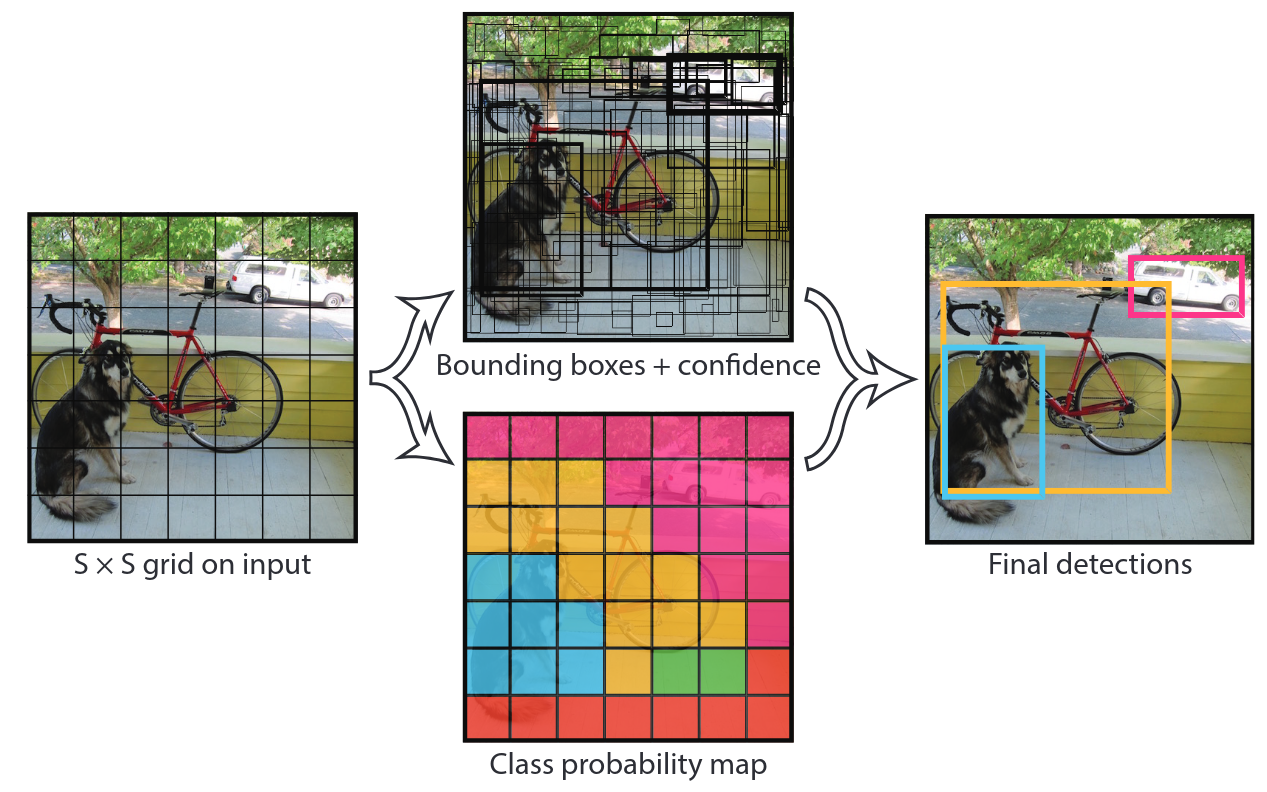
\includegraphics[scale=0.25]{figures/YOLO_functionality.png}
	\caption{YOLO}
\end{figure}
